\documentclass[a4paper,cs4size]{BHCexam}
%\documentclass[a4paper,cs4size,answers]{BHCexam}

\usepackage{multicol} % 分栏
\pagestyle{fancy}
\fancyfoot[C]{\kaishu \small 第 \thepage 页 共 \pageref{lastpage} 页}
%\fancyhead[L]{\includegraphics[width=2cm]{qrcode.png}}
\title{压力压强习题课}
%\subtitle{数学文科试卷}
%\notice{满分150分, 120分钟完成, \\	允许使用计算器,答案一律写在答题纸上.}
%\author{Gavin Chen}
%\date{\today}

\begin{document}
\maketitle
\begin{groups}
    \group{}{}
    \zihao{-4}
    \begin{questions}[]

        \question[5] 如图所示,一实心均匀柱体静止在水平地面上。已知柱体的高为$0.4m$,柱体的底面积为$0.01m^2$,柱体的质量为$8kg$。求:
        \begin{subquestions}
            \subquestion 柱体对水平地面的压力和压强。
            \subquestion 现将柱体沿水平方向切去$0.1m$的高度,求柱体对地面的压强变化量。
        \end{subquestions}
        \begin{figure}[htb]
            \flushright
            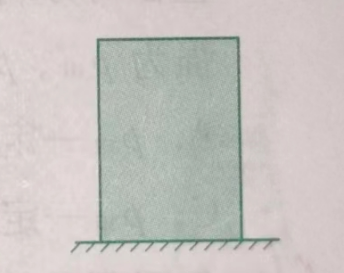
\includegraphics [scale=0.4,trim=0 0 0 0]{./image/physics_pressure_1.png}
            % \caption{图名}
            \label{fig:fig_pressure_1}
        \end{figure}
        \begin{solution}{0.5cm}
            \methodonly 略
        \end{solution}
        \vspace{5cm}

        \question[5] 质量相等的甲、乙两个均匀圆柱体放置在水平地面上。现沿水平虚线切去部分后,使甲、乙剩余部分的高度相等,
        如图所示,则它们剩余部分对地面压强$p_{\text{甲}},p_{\text{乙}}$和压力$F_{\text{甲}},F_{\text{乙}}$的关系是(\quad\quad\quad)。
        \fourchoices{$p_{\text{甲}}<p_{\text{乙}},\quad F_{\text{甲}}<F_{\text{乙}}$}
        {$p_{\text{甲}}<p_{\text{乙}},\quad F_{\text{甲}}>F_{\text{乙}}$}
        {$p_{\text{甲}}>p_{\text{乙}},\quad F_{\text{甲}}<F_{\text{乙}}$}
        {$p_{\text{甲}}>p_{\text{乙}},\quad F_{\text{甲}}>F_{\text{乙}}$}
        \begin{figure}[htb]
            \flushright
            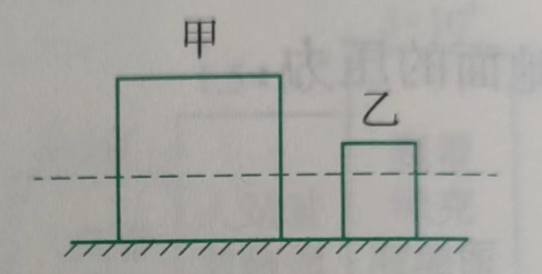
\includegraphics [scale=0.4,trim=0 0 0 0]{./image/physics_pressure_2.png}
            % \caption{图名}
            \label{fig:fig_pressure_2}
        \end{figure}
        \vspace{5cm}

        \question[5] 如图所示,在质量、高度均相等的甲、乙两圆柱体上沿水平方向切去相同的厚度,
        并将切去部分叠放至对方剩余部分上表面的中央。若此时甲'、乙'对地面的压力、压强分别
        为$F'_{\text{甲}},F'_{\text{乙}}$和$p'_{\text{甲}},p'_{\text{乙}}$,则(\quad\quad\quad)。
        \fourchoices{$F'_{\text{甲}}>F'_{\text{乙}},\quad p'_{\text{甲}}>p'_{\text{乙}}$}
        {$F'_{\text{甲}}<F'_{\text{乙}},\quad p'_{\text{甲}}>p'_{\text{乙}}$}
        {$F'_{\text{甲}}=F'_{\text{乙}},\quad p'_{\text{甲}}=p'_{\text{乙}}$}
        {$F'_{\text{甲}}=F'_{\text{乙}},\quad p'_{\text{甲}}>p'_{\text{乙}}$}
        \begin{figure}[htb]
            \flushright
            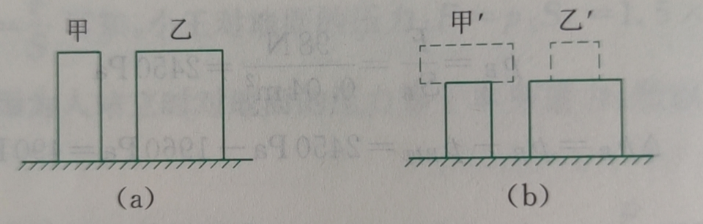
\includegraphics [scale=0.4,trim=0 0 0 0]{./image/physics_pressure_3.png}
            % \caption{图名}
            \label{fig:fig_pressure_3}
        \end{figure}
        \vspace{5cm}

        \question[5] 如图所示,甲、乙、丙、丁是四个完全相同的圆柱体竖放在水平地面上,若把乙、丙、丁中的阴影部分切除后,
        则甲、乙、丙、丁对水平地面的压强大小关系正确的是(\quad\quad\quad)。
        \fourchoices{$p_{\text{丁}}<p_{\text{甲}}=p_{\text{乙}}<p_{\text{丙}}$}
        {$p_{\text{甲}}=p_{\text{乙}}<p_{\text{丁}}<p_{\text{丙}}$}
        {$p_{\text{甲}}>p_{\text{乙}}>p_{\text{丙}}>p_{\text{丁}}$}
        {$p_{\text{丁}}<p_{\text{甲}}<p_{\text{乙}}=p_{\text{丙}}$}
        \begin{figure}[htb]
            \flushright
            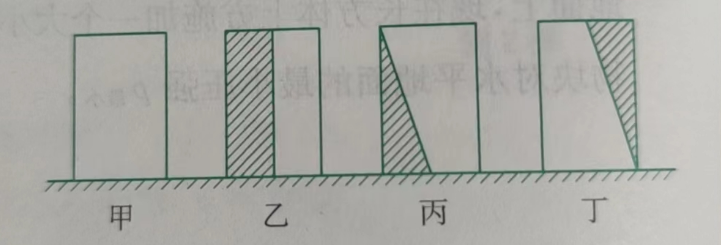
\includegraphics [scale=0.4,trim=0 0 0 0]{./image/physics_pressure_4.png}
            % \caption{图名}
            \label{fig:fig_pressure_4}
        \end{figure}
        \vspace{5cm}

        \question[5] 如图所示,底面积不同的圆柱形容器$A$和$B$分别盛有甲、乙两种液体,
        两液面相平,且甲的质量大于乙的质量。若在两容器中分别加入原有液体后,液面高度仍保持相平,
        则此时液体对各自容器底部的压强$p_A, p_B$和压力$F_A, F_B$的大小关系是(\quad\quad\quad)。
        \fourchoices{$p_A<p_B, \quad F_A=F_B$}
        {$p_A<p_B, \quad F_A>F_B$}
        {$p_A>p_B, \quad F_A=F_B$}
        {$p_A>p_B, \quad F_A>F_B$}
        \begin{figure}[htb]
            \flushright
            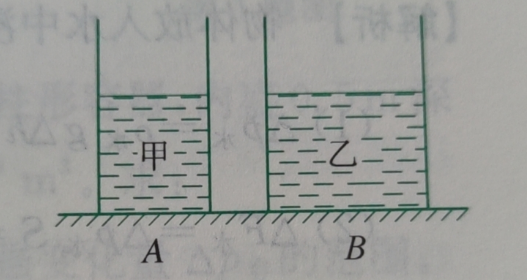
\includegraphics [scale=0.4,trim=0 0 0 0]{./image/physics_pressure_5.png}
            % \caption{图名}
            \label{fig:fig_pressure_5}
        \end{figure}
        \vspace{5cm}

        \question[5] 如图所示,底面积不同的圆柱形容器分别盛有甲、乙两种液体,液体对各自容器底部的压强相等。
        若在两容器中分别抽出相同高度的液体,则剩余液体对各自容器底部的压强$p$、压力$F$的大小关系是(\quad\quad\quad)。
        \fourchoices{$p_{\text{甲}}>p_{\text{乙}},\quad F_{\text{甲}}>F_{\text{乙}}$}
        {$p_{\text{甲}}<p_{\text{乙}},\quad F_{\text{甲}}<F_{\text{乙}}$}
        {$p_{\text{甲}}=p_{\text{乙}},\quad F_{\text{甲}}>F_{\text{乙}}$}
        {$p_{\text{甲}}=p_{\text{乙}},\quad F_{\text{甲}}<F_{\text{乙}}$}
        \begin{figure}[htb]
            \flushright
            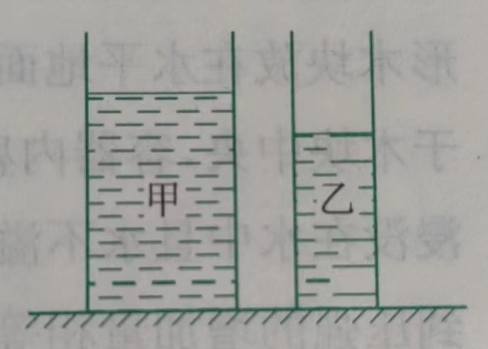
\includegraphics [scale=0.4,trim=0 0 0 0]{./image/physics_pressure_6.png}
            % \caption{图名}
            \label{fig:fig_pressure_6}
        \end{figure}
        \vspace{5cm}

        \question[5] 如图所示,实心均匀正方体甲、乙对水平地面的压强相同。现沿竖直方向切去相同体积,
        并将切去部分放置在对方剩余部分的上表面,若此时它们对地面的压强为$p_{\text{甲}},p_{\text{乙}}$,则(\quad\quad\quad)。
        \fourchoices{$p_{\text{甲}}$一定大于$p_{\text{乙}}$}
        {$p_{\text{甲}}$可能小于$p_{\text{乙}}$}
        {$p_{\text{甲}}$一定等于$p_{\text{乙}}$}
        {$p_{\text{甲}}$可能等于$p_{\text{乙}}$}
        \begin{figure}[htb]
            \flushright
            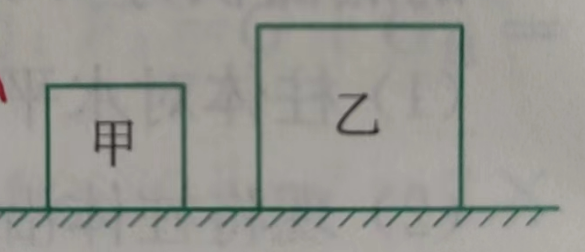
\includegraphics [scale=0.4,trim=0 0 0 0]{./image/physics_pressure_7.png}
            % \caption{图名}
            \label{fig:fig_pressure_7}
        \end{figure}
        \vspace{6.5cm}

        \question[5] 重为$2N$、底面积为$1\times 10^{-2}m^2$的薄壁柱形容器内盛有$0.2m$深的水,放在水平面上。
        若在容器中浸没一密度为$2.5\times 10^3kg/m^3$,体积为$2\times 10^{-4}m^3$的物块,且无水溢出。求:
        \begin{subquestions}
            \subquestion 水对容器底的压强增加量。
            \subquestion 水对容器底的压力增加量。
            \subquestion 容器对桌面的压力增加量。
            \subquestion 容器对桌面的压强增加量。
        \end{subquestions}
        \vspace{6.5cm}

        \question[5] 如图所示,质量为$0.1kg$、底面积为$1\times 10^{-2}m^2$的正方形木块放在水平地面上,
        底面积为$5\times 10^{-3}m^2$的柱形轻质容器置于木块中央,容器内盛有$0.4kg$的水。在水中放入一物块,
        物块浸没在水中且水不溢出,若水对容器底部压强的增加量与地面受到压强的增加量相等,求物块的密度$\rho_{\text{物}}$。
        \begin{figure}[htb]
            \flushright
            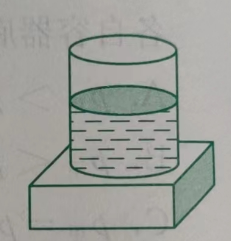
\includegraphics [scale=0.4,trim=0 0 0 0]{./image/physics_pressure_8.png}
            % \caption{图名}
            \label{fig:fig_pressure_8}
        \end{figure}
        \vspace{6.5cm}

        \question[5] 如图所示,盛有液体甲的轻质圆柱形容器和均匀圆柱体乙放置在水平地面上,
        甲、乙对地面的压强相等。现从容器中抽出部分液体甲并沿水平方向切去部分乙后,
        甲、乙剩余部分的体积相等。若甲、乙减少的质量分别为$m_{\text{甲}}, m_{\text{乙}}$,则(\quad\quad\quad)。
        \fourchoices{$m_{\text{甲}}$一定小于$m_{\text{乙}}$}
        {$m_{\text{甲}}$一定等于$m_{\text{乙}}$}
        {$m_{\text{甲}}$一定大于$m_{\text{乙}}$}
        {$m_{\text{甲}}$可能小于$m_{\text{乙}}$}
        \begin{figure}[htb]
            \flushright
            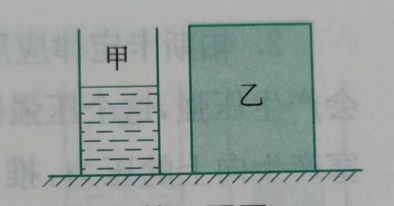
\includegraphics [scale=0.4,trim=0 0 0 0]{./image/physics_pressure_9.png}
            % \caption{图名}
            \label{fig:fig_pressure_9}
        \end{figure}
        \vspace{5cm}

        \question[5] 水平地面上有一个底面积为$2\times 10^{-2}m^2$的轻质薄壁柱形容器,内盛$0.5m$深
        的水,一个实心金属球的质量为$3kg$,体积为$1\times 10^{-3}m^3$。求:
        \begin{subquestions}
            \subquestion 将金属球浸没在容器内的水中,容器对桌面的压强变化量$\Delta p_{\text{容}}$的范围。
            \subquestion 将金属球浸没在容器内的水中,液体对容器底部的压强变化量$\Delta p_{\text{液}}$液的范围。
        \end{subquestions}


    \end{questions}





\end{groups}


\label{lastpage}
\end{document}
